\section{Figures}

% first figure
\begin{figure}[H]

\includegraphics[width=\linewidth]{img1.jpg}
\caption{Your first figure placement}
\end{figure}

% second figure
\blindtext 
\begin{wrapfigure}{r}{0.5\textwidth}
	\begin{center}
		
\includegraphics[width=0.48\textwidth]{img2.jpg}
	\end{center}
	\caption{Wrapped around}
\end{wrapfigure}
\blindtext 

% third figure
\begin{figure}[H]
    \centering
    \begin{subfigure}[b]{0.3\textwidth}
        
\includegraphics[width=\textwidth]{img1.jpg}
        \caption{caption 1}
    \end{subfigure}
	% space
    \begin{subfigure}[b]{0.3\textwidth}
        
\includegraphics[width=\textwidth]{img2.jpg}
        \caption{caption 2}
    \end{subfigure}
    % space
    \begin{subfigure}[b]{0.3\textwidth}
        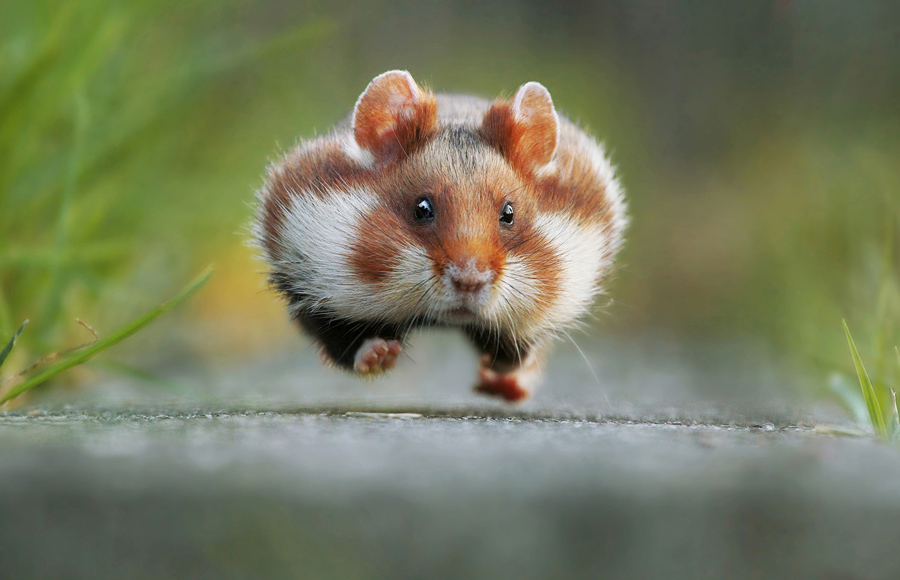
\includegraphics[width=\textwidth]{img3.jpg}
        \caption{caption 3}
    \end{subfigure}
    \caption{Pictures of cute things}
\end{figure}